\subsection{Searcher}
\label{subsec:searcher}

In the searcher we have used a \emph{boolean query} approach, in this way it was possible to create complex queries by combining, using the \emph{boolean operators}, different components to be matched. The components we have used in our queries are explained from Section~\ref{subsubsec:bm25} to Section~\ref{subsubsec:reranker}. Note that in the following, the word N-grams component explained in Section~\ref{subsubsec:shingles} will be referenced also with the Lucene's jargon \emph{shingles}.

\subsubsection{BM25}
\label{subsubsec:bm25}

Since the document collection has a significant size, as a base of our system we opted for a classic BM25\citep{RobertsonZaragoza2009} approach due to the \emph{efficiency} of it and higher \emph{effectiveness} compared to other methods.  \\
The Lucene \citep{Lucene} implementation has default values $k1=1.2$ and $b=0.75$ which worked fine, but we decided to fine-\emph{tune} the parameters to improve measures, in particular, \ac{nDCG} since it is the relevant measure for the LongEval campaign. The results of our experiments are reported in Table~\ref{tab:BM25}.

\begin{table}[!h]
% Please add the following required packages to your document preamble:
% \usepackage{multirow}
% \usepackage[table,xcdraw]{xcolor}
% If you use beamer only pass "xcolor=table" option, i.e. \documentclass[xcolor=table]{beamer}
\begin{tabular}{|cc|cccccccc|}
\toprule
\multicolumn{2}{|l|}{\textbf{Run}} & \multicolumn{8}{c|}{FADERIC\_French-Stop50-Stem-Shingle-Fuzzy}\\
\midrule
\multicolumn{2}{|l|}{\textbf{Measure}} & \multicolumn{8}{c|}{ndcg}\\
\midrule
& \multicolumn{1}{l|}{}    & \multicolumn{8}{c|}{\textbf{k1}}\\
\cmidrule{3-10}
 & \multicolumn{1}{l|}{}  & \multicolumn{1}{l|}{0.6} & \multicolumn{1}{l|}{0.8} & \multicolumn{1}{l|}{1.0} & \multicolumn{1}{l|}{1.2} & \multicolumn{1}{l|}{1.4} & \multicolumn{1}{l|}{1.6} & \multicolumn{1}{l|}{1.8}   & \multicolumn{1}{l|}{2.0} \\
\midrule
\multicolumn{1}{|c|}{}                             & 0,30                      & \multicolumn{1}{c|}{\cellcolor[HTML]{E27066}0,3941} & \multicolumn{1}{c|}{\cellcolor[HTML]{E67F66}0,3952} & \multicolumn{1}{r|}{\cellcolor[HTML]{E78266}0,3954} & \multicolumn{1}{c|}{\cellcolor[HTML]{E88766}0,3957} & \multicolumn{1}{c|}{\cellcolor[HTML]{EB8F66}0,3963} & \multicolumn{1}{c|}{\cellcolor[HTML]{E06866}0,3936}          & \multicolumn{1}{c|}{\cellcolor[HTML]{E57A66}0,3948}          & \cellcolor[HTML]{E06666}0,3934 \\ %\cmidrule{2-10} 
\multicolumn{1}{|c|}{}                             & 0,40                      & \multicolumn{1}{c|}{\cellcolor[HTML]{EC9566}0,3967} & \multicolumn{1}{c|}{\cellcolor[HTML]{F1A866}0,398}  & \multicolumn{1}{c|}{\cellcolor[HTML]{F3AD66}0,3984} & \multicolumn{1}{c|}{\cellcolor[HTML]{F6B966}0,3992} & \multicolumn{1}{c|}{\cellcolor[HTML]{F6B966}0,3992} & \multicolumn{1}{c|}{\cellcolor[HTML]{F6B966}0,3992}          & \multicolumn{1}{c|}{\cellcolor[HTML]{F2A966}0,3981}          & \cellcolor[HTML]{EFA066}0,3975 \\ %\cmidrule{2-10} 
\multicolumn{1}{|c|}{}                             & 0,50                      & \multicolumn{1}{c|}{\cellcolor[HTML]{F9C366}0,3999} & \multicolumn{1}{c|}{\cellcolor[HTML]{FBCA66}0,4004} & \multicolumn{1}{c|}{\cellcolor[HTML]{FCD066}0,4008} & \multicolumn{1}{c|}{\cellcolor[HTML]{FED766}0,4013} & \multicolumn{1}{c|}{\cellcolor[HTML]{FFD966}0,4014} & \multicolumn{1}{c|}{\cellcolor[HTML]{FFD966}0,4014}          & \multicolumn{1}{c|}{\cellcolor[HTML]{FFD966}0,4014}          & \cellcolor[HTML]{FDD466}0,4011 \\ %\cmidrule{2-10} 
\multicolumn{1}{|c|}{}                             & 0,60                      & \multicolumn{1}{c|}{\cellcolor[HTML]{F9C366}0,3999} & \multicolumn{1}{c|}{\cellcolor[HTML]{FED766}0,4013} & \multicolumn{1}{c|}{\cellcolor[HTML]{F2D564}0,4017} & \multicolumn{1}{c|}{\cellcolor[HTML]{CEC95F}0,4025} & \multicolumn{1}{c|}{\cellcolor[HTML]{C9C85E}0,4026} & \multicolumn{1}{c|}{\cellcolor[HTML]{D2CB60}0,4024}          & \multicolumn{1}{c|}{\cellcolor[HTML]{E9D263}0,4019}          & \cellcolor[HTML]{FCD066}0,4008 \\ %\cmidrule{2-10} 
\multicolumn{1}{|c|}{}                             & 0,70                      & \multicolumn{1}{c|}{\cellcolor[HTML]{E0CF62}0,4021} & \multicolumn{1}{c|}{\cellcolor[HTML]{BCC35C}0,4029} & \multicolumn{1}{c|}{\cellcolor[HTML]{A5BC59}0,4034} & \multicolumn{1}{c|}{\cellcolor[HTML]{93B656}0,4038} & \multicolumn{1}{c|}{\cellcolor[HTML]{7DAE52}0,4043} & \multicolumn{1}{c|}{\cellcolor[HTML]{6AA84F}\textbf{0,4047}} & \multicolumn{1}{c|}{\cellcolor[HTML]{6FAA50}0,4046}          & \cellcolor[HTML]{8FB455}0,4039 \\ %\cmidrule{2-10} 
\multicolumn{1}{|c|}{}                             & 0,75                     & \multicolumn{1}{c|}{\cellcolor[HTML]{EDD464}0,4018} & \multicolumn{1}{c|}{\cellcolor[HTML]{C0C55D}0,4028} & \multicolumn{1}{c|}{\cellcolor[HTML]{A1BA58}0,4035} & \multicolumn{1}{c|}{\cellcolor[HTML]{8FB455}0,4039} & \multicolumn{1}{c|}{\cellcolor[HTML]{93B656}0,4038} & \multicolumn{1}{c|}{\cellcolor[HTML]{7DAE52}0,4043}          & \multicolumn{1}{c|}{\cellcolor[HTML]{98B756}0,4037}          & \cellcolor[HTML]{A1BA58}0,4035 \\ %\cmidrule{2-10} 
\multicolumn{1}{|c|}{}                             & 0,80 & \multicolumn{1}{c|}{\cellcolor[HTML]{FDD366}0,401}  & \multicolumn{1}{c|}{\cellcolor[HTML]{CEC95F}0,4025} & \multicolumn{1}{c|}{\cellcolor[HTML]{AABD59}0,4033} & \multicolumn{1}{c|}{\cellcolor[HTML]{8AB354}0,404}  & \multicolumn{1}{c|}{\cellcolor[HTML]{86B154}0,4041} & \multicolumn{1}{c|}{\cellcolor[HTML]{7DAE52}0,4043}          & \multicolumn{1}{c|}{\cellcolor[HTML]{6AA84F}\textbf{0,4047}} & \cellcolor[HTML]{8FB455}0,4039 \\ %\cmidrule{2-10} 
\multicolumn{1}{|c|}{\multirow{-8}{*}{\textbf{b}}} & 0,90 & \multicolumn{1}{c|}{\cellcolor[HTML]{F3AF66}0,3985} & \multicolumn{1}{c|}{\cellcolor[HTML]{F8C266}0,3998} & \multicolumn{1}{c|}{\cellcolor[HTML]{FDD166}0,4009} & \multicolumn{1}{c|}{\cellcolor[HTML]{FFD966}0,4014} & \multicolumn{1}{c|}{\cellcolor[HTML]{EDD464}0,4018} & \multicolumn{1}{c|}{\cellcolor[HTML]{E0CF62}0,4021}          & \multicolumn{1}{c|}{\cellcolor[HTML]{FBD866}0,4015}          & \cellcolor[HTML]{FDD466}0,4011 \\
\bottomrule
\end{tabular}
\caption{\label{tab:BM25} NDCG results with different BM25 parameters}
\end{table}
The best result was given by two pairs: $k1=1.8, b=0.8$ and $k1=1.6, b=0.7$; we chose pair $k1=1.8, b=0.8$ due to having the highest \ac{MAP}.  Note that the performance gain was minimal, just $0,006$ from the score with default parameters, which was expected.

\subsubsection{Fuzzy}
\label{subsubsec:fuzzy}


A \emph{fuzzy} search, or approximate search, is a technique used to search for approximate or \emph{partial} matches between a search term and documents in a collection of texts. Unlike exact search, in which the match must be exact and precise, fuzzy search allows you to find results even when the words you search for do not exactly match those in the documents.
Fuzzy search is particularly useful when you want to get results even if there are \emph{misspellings}, \emph{language variants}, \emph{abbreviations} or other forms of variations in the search terms or texts of the documents. For example, if you search for the term "roam" with a fuzzy search, the document containing the term "foam" might also be returned.

Fuzzy search techniques are based on the use of algorithms that evaluate the similarity between text strings. One of the most common algorithms used for fuzzy search is the Levenshtein algorithm \citep{levenshtein1966binary}, which calculates the editing distance between two strings, that is, the minimum number of operations (insertions, deletions, and character substitutions) required to transform one string into the other. Lucene \citep{Lucene}, for example, uses a variant of the algorithm just described, the Damerau-Levenshtein algorithm, named after the Damerau algorithm \citep{damerau1964technique}.

Lucene \citep{Lucene} also allows you to add an additional (optional) parameter with which to specify the maximum number of changes allowed. In our case we decided to set a manual \emph{threshold} to choose the value of the parameter; if the word length is greater than or equal to the threshold then the fuzzy parameter is set to 2 otherwise 1 is used. The threshold is called "fuzzyThreshold" and can be set in the configuration file; we decided to set it to 10.
Finally, to avoid performance degradation, in our IR system, fuzzy search is applied only if the query contains a single term.


\subsubsection{Shingles}
\label{subsubsec:shingles}

Shingles are a sentence analysis technique of dividing the words of a sentence into sequences of $n$ consecutive words. For example, for the sentence "the dog barks," we can create the n-grams "the dog" and "dog barks." Shingles are useful because they capture \emph{local relationships} between words within a text, so this approach helps identify similar, though not identical, phrases and can \emph{improve search relevance}.
The maximum number of words within a shingle can be set in the configuration file in \texttt{maxShingleSize}; in our case, we decided to generate shingles with a maximum of 3 words. Also, we avoided generating unigrams, i.e., shingles with exactly one word, as they do not capture any local relationships within the query.

We then decided to set up a proximity search within each shingle. The proximity of terms in a shingle can be used to identify documents in which the search terms occur in a certain \emph{spatial relationship}.
For example, if we are searching for the terms "dog" and "brown" with the proximity of 3 words, we want to find documents in which these two terms appear within a maximum distance of three words from each other. Thus, if a document contains sentences such as "I saw a brown dog in the park" or "The brown dog was running fast," these documents would be considered relevant because the terms "dog" and "brown" are close to each other. In our case, the proximity parameter is set to 5.

Finally, we applied a boost to all shingles based on the size of the shingle itself.


\subsubsection{Synonyms}
\label{subsubsec:synonyms}

Managing synonyms in a retrieval system is not straightforward. The use of synonyms may not necessarily improve results, and this depends on how they are used.

Synonyms may be useful in the context of \ac{IR} to broaden the search to include more related terms. However, the introduction of synonyms can also create problems such as noise in the information retrieval process. Here are some reasons why the use of synonyms may not improve results:
\begin{itemize}
	\item \textbf{Polysemy}: words may have \emph{more than one meaning}. Introducing synonyms might lead to an increase in irrelevant results if a synonym is associated with another meaning of the searched word. For example, if one searches for "bank" in the context of a financial bank, introducing the synonym "riverbank" could generate irrelevant results.
	\item \textbf{Irrelevant synonyms}: not all synonyms are equally \emph{relevant in the context} of a given query. Some synonyms might be too general or too specific concerning the user's intent, leading to inappropriate or insufficient results.
	\item \textbf{Redundancy}: adding synonyms can lead to redundancy in the answers provided. If multiple synonymous words or phrases are used in the query, there may be significant overlap between the results, reducing the overall effectiveness of the IR system.
\end{itemize}

However, it should be kept in mind that the effectiveness of using synonyms in improving the results of the IR system also depends on the specific implementation and the characteristics of the domain or context in which the system is used. In some cases, the use or \emph{expansion} of synonyms could actually improve the accuracy of information retrieval. 

Furthermore, the use of synonyms can increase computational complexity in the information retrieval process. Because synonyms require accurate correspondence with indexed documents, additional computations must be performed to identify and compare matching synonyms in indexed texts. \\

We made several attempts to implement synonyms in our system; a summary description of what we did is given below.

Firstly, since handling synonyms in the index takes too much computation time, we decided to handle them directly in the search. We added synonyms in the queries with a query expansion approach. \\

In addition, we decided to use the WordNet dictionary\citep{wordNet}. WordNet is a lexical database that groups English words into sets of synonyms called synsets, providing semantic relationships and definitions. It offers a comprehensive resource for natural language processing tasks, such as word sense disambiguation, information retrieval, and sentiment analysis.
Since WordNet is written in C, it was necessary to use an additional API in order to use the dictionary on our system. That API is called extJWNL (Extended Java WordNet Library)\citep{extJWNL} and does not need the WordNet database installed locally. \\

Also, to improve dictionary lookup, we decided to use the OpenNLP \citep{OpenNLP} library for natural language processing and limit polysemy. Each word in the original query was processed by an OpenNLP \ac{PoS} Tagger in order to obtain the tag associated with the word. That function analyzes the context in which the word is used and returns the associated tag. The model used for the pos tagger was \texttt{en-pos-maxent.bin} and the tags are associated with WordNet section as shown in Table \ref{tab:opennlp-tags}.\\
Knowing the tag of each word in a query made it possible to look up the word in the corresponding dictionary section. For example, for the query "free software," free was searched in the adjective section and software in the noun section.
This strategy improved the metrics very little probably because the queries provided by Long Eval are very short, averaging 2/3 words. In addition, OpenNLP works well with \emph{properly formulated sentences}, including consideration of capitalization and punctuation. In this case, queries are very crudely formulated, for example, some begin with a capital letter and some do not, as a result, OpenNLP does not always provide the correct tag. Then, this strategy might be more useful in the case of more complex queries, such as those characterizing a conversational \ac{IR} system. \\

\begin{table}[h]
    \caption{OpenNLP Tags compared with WordNet Sections}
    \label{tab:opennlp-tags}
    \centering
    \begin{tabular}{|c|c|}
        \toprule
        \textbf{OpenNLP Tag} & \textbf{WordNet Section}\\
        \midrule
        JJ & Adjectives\\
        
        VB & Verbs\\
        
        RB & Adverbs\\
        
        NN & Nouns\\
        
        Others & No synonyms retrieved\\
        \bottomrule
    \end{tabular}
\end{table}

Subsequently, we tried to give a \emph{different boost} to each synonym. As a first approach, we decided to provide a boost based on the amount of synonyms returned. In this case, the boost was calculated in this way: 
\begin{equation}
boost=\frac{Boost Base}{Synonym List Length}
\end{equation}
This approach was used to limit the importance associated with each synonym if the returned synonym list is long, being more likely to get \emph{irrelevant synonyms}. \\

Finally, we moved synonym management, creating two new Analyzers: \texttt{SynonymAnalyzer} and \texttt{SynonymPOSAnalyzer}, which are applied only in the search part:
\begin{itemize}
	\item \textbf{\texttt{SynonymAnalyzer}}: uses as input a query already previously analyzed with the standard Analyzer, i.e. \texttt{EnglishLongEvalAnalyzer} or \texttt{FrenchLongEvalAnalyzer}, after applies: \texttt{SynonymGraphFilter}, \texttt{FlattenGraphFilter} and \texttt{StopFilter}.\\ 
\texttt{SynonymGraphFilter} represents a filter that can be directly applied to a \texttt{TokenStream} within an Analyzer. The filter creates a synonym graph based on specified configurations and expands the terms found in the analyzed text by adding the corresponding synonyms to the token graph. \texttt{FlattenGraphFilter} converts an incoming graph token stream, such as one from \texttt{SynonymGraphFilter}, into a flat form so that all nodes form a single linear chain with no side paths. Every path through the graph touches every node. This is necessary when indexing a graph token stream because the index does not save \texttt{PositionLengthAttribute} and so it cannot preserve the graph structure. However, at search time, query parsers can correctly handle the graph and this token filter should not be used.

This Analyzer uses a list of synonyms in .txt format, available in two versions: standard and custom. Before being processed by the Analyzer, the synonym list is transformed into a \texttt{SynonymMap} object via the \texttt{AnalyzerUtil}'s \texttt{loadSynonymList} function. \\

	\item \textbf{\texttt{SynonymPOSAnalyzer}}: takes as input \texttt{EnglishLongEvalAnalyzer}, then applies an \texttt{OpenNLPPOSFilter}, so that each word is assigned the associated tag.
Then, it applies a custom filter called \texttt{SynonymPOSFilter} to manage the tags and look up words in the WordNet dictionary. Creating a custom filter was not trivial as the information about it in the documentation and online is very limited. 
The filter allows us to:
	\begin{enumerate}
		\item fetch the input tokens, 
		\item retrieve their associated tag, 
		\item search the synonyms in the dictionary based on their tag,
		\item process the synonyms with the standard analyzer i.e. \texttt{EnglishLongEvalAnalyzer}
		\item and return as output a TokenStream containing all the synonyms found. 
	\end{enumerate}
\end{itemize}
The tokenStream returned as output by both Analyzers is then transformed into a list of strings which is in turn processed by the \texttt{Searcher} to apply a boost. Finally, the synonyms are added to the \texttt{BooleanQuery} along with the original query.

\subsubsection{Reranker}
\label{subsubsec:reranker}

After all of the previous steps, we obtained a working system that achieved decent results at a good speed, so we tried to improve it by introducing a second stage, called \textit{passage re-ranking}, in which each of the documents returned by the first retrieval model would be scored and re-ranked by a more computationally-intensive method involving Machine Learning. \\
\begin{figure}[!h]
  \centering
  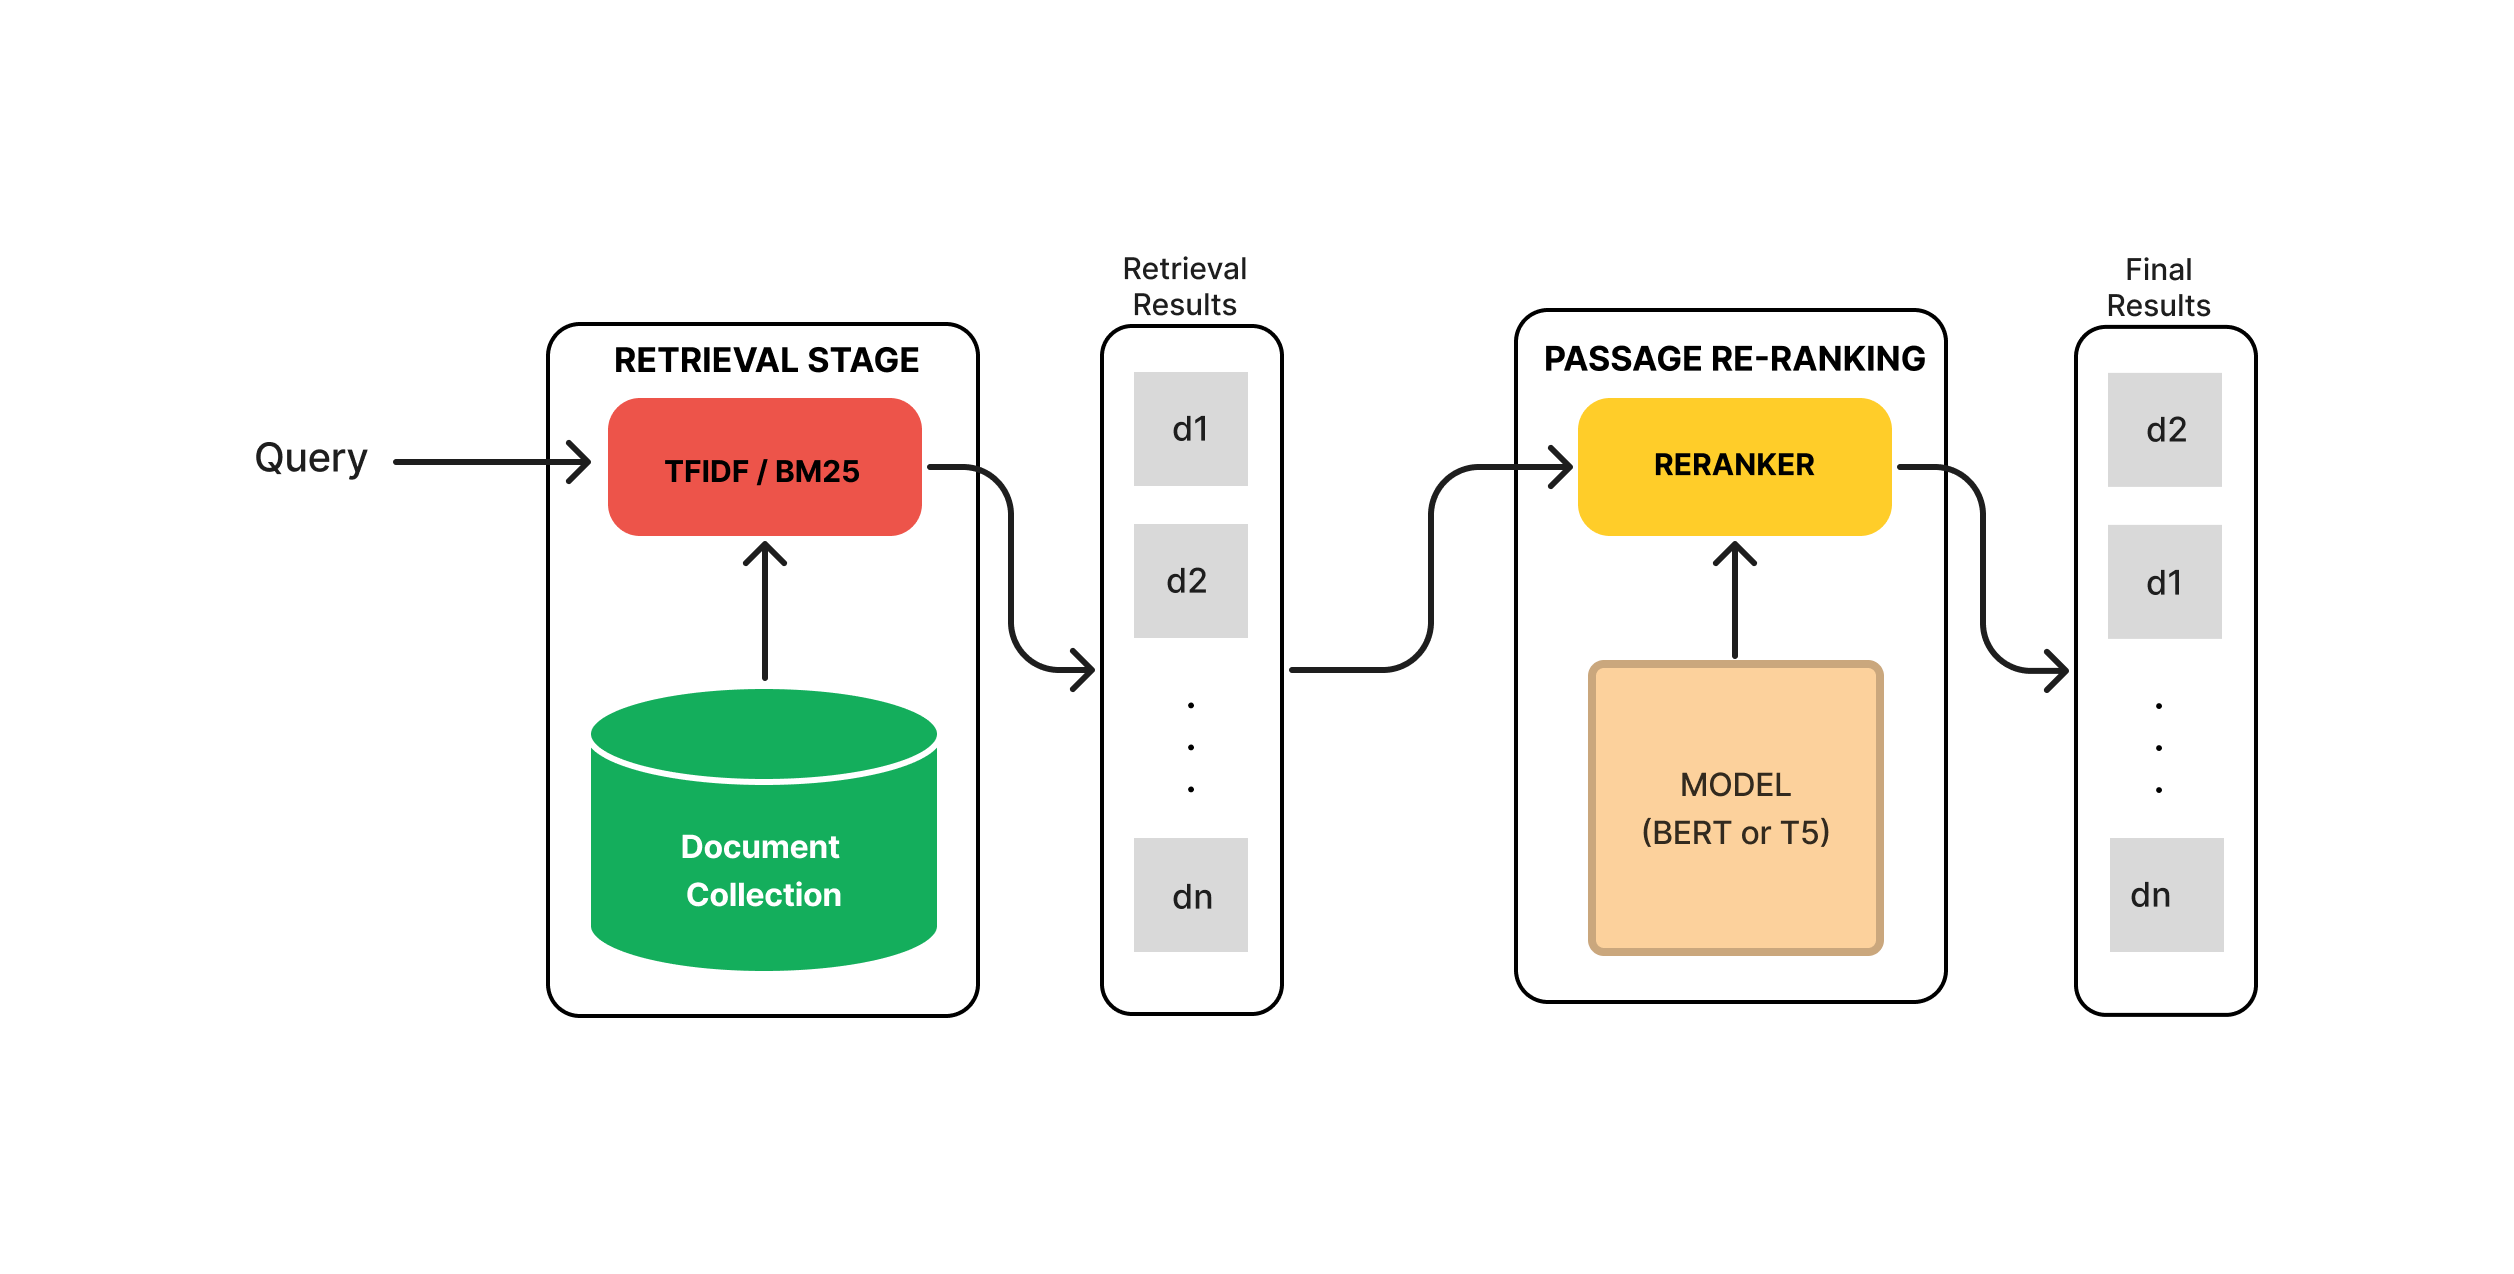
\includegraphics[width=0.8\linewidth]{figure/rerank_framework.png}
  \caption{Retrieve-than-rerank framework}
  \label{fig:rerank}
\end{figure}
We achieved this by leveraging a library called PyGaggle\cite{pygaggle}, which provides some deep neural architectures for text ranking and question answering, and two transformer-based models, T5 and BERT, with different checkpoints and even our own trained checkpoint using code from another library\cite{gao2021lce}. \\

In our system, we can choose how many documents are to be reranked from the top for two reasons: the first is raw computing performance, reranking all 1000 retrieved documents takes a long time and we don't have machines powerful enough to handle it; the second is that we saw that reranking more than 50 documents drops our measures down, even below the baseline measure without reranking.\\
Our first approach to reranking was to consider only the scores returned by the models to rerank the documents but we then switched to an approach where we consider also the BM25 score as follows. Let $Score_{BM25}(i)$ the score given by BM25 for the document at rank $i$ and $Score_{rr}(i)$ the score given by the reranker for the document at rank $i$, and let $n$ be the total number of reranked documents, we define: 
\begin{equation}
nScore_{rr}(i) = \bigg(Score_{rr}(i)+\min_{j\in [1,n]}Score(j)\bigg)\cdot \frac{Score_{BM25}(1)}{Score_{rr}(1)}
\end{equation}
as the normalized score for the reranked documents, since the models returned a score in the range $[-10,+10]$, which was not suitable for our case.\\
In our first approach, we simply passed the score to Lucene's \texttt{ScoreDoc} object and we were done. But in this way, we would lose information about the ranking given by BM25, which is still relevant, so we defined a new score: 
\begin{equation}
finalScore(i) = mntr + (1-\alpha)\cdot Score_{BM25}(i)+\alpha\cdot nScore_{rr}(i)
\end{equation}
where $mntr$ is the maximum score from docs which are not reranked, in this way, we preserve the order of this docs. With this approach, we can give a weight to the reranker to find the balance and we do not lose the information given to us by the first stage. Note that $\alpha=1$ corresponds to considering only scores from the reranker. \\

\noindent \textbf{Pretrained Models}

We tried two transformer-based models, T5 and BERT since they are supported by PyGaggle. First, we tried T5\cite{RaffelShazeerRobertsLeeNarangMatenaZhouLiLiuT5}, but with BERT\cite{devlin2019bert} we got better results. Starting from the same base model, t5-base\cite{t5base} for T5 bert-base-uncased\cite{bertbase} for BERT, we tried different checkpoints\footnote{saving the model's parameters and optimizer state during the training process} fine-tuned specifically for reranking tasks and we even tried to train our checkpoint. The pre-trained checkpoints that we used are: 
\begin{itemize}
\item \textit{monot5-base-msmarco-10k}\cite{castorinimonot5}
\item \textit{bert-base-mdoc-bm25}\cite{bertbasebm25}
\end{itemize}
The results for the T5 model are reported in Table~\ref{tab:t5-msmarco} and the results for the BERT model are reported in Table~\ref{tab:bert-mdoc}.
\begin{table}[!h]
\caption{\label{tab:t5-msmarco} monot5-base-msmarco-10k model with different number of documents to rerank}
\begin{tabular}{|l|l|l|}
\toprule
             & \textbf{nDCG} & \textbf{map} \\ 
\midrule
\textbf{0}   & 0,4075        & 0,2411       \\ 
\textbf{10}  & \textbf{0,414}         & \textbf{0,2502}       \\ 
\textbf{20}  & 0,4119        & 0,2477       \\ 
\textbf{50}  & 0,4083        & 0,242        \\ 
\textbf{100} & 0,405         & 0,2376       \\ 
\textbf{250} & 0,3987        & 0,2301\\
\bottomrule
\end{tabular}
\end{table}

\begin{table}[!h]
\caption{\label{tab:bert-mdoc}bert-base-mdoc-bm25 model with different number of documents to rerank}
\begin{tabular}{|l|l|l|}
\toprule
             & \textbf{nDCG} & \textbf{map} \\ 
\midrule
\textbf{0}   & 0,4075        & 0,2411       \\ 
\textbf{10}  & 0,4207         & 0,2608       \\ 
\textbf{20}  & \textbf{0,4222}        & \textbf{0,2617}       \\ 
\textbf{50}  & 0,4212        & 0,2598        \\ 
\textbf{100} & 0,4184         & 0,2563       \\ 
\textbf{250} & 0,4104        & 0,2478      \\
\bottomrule
\end{tabular}
\end{table}
The BERT pretrained checkpoint with 20 reranked documents improved \ac{nDCG} by $3.56\%$ and \ac{MAP} by $8.5\%$.\\

\noindent \textbf{Training our own checkpoint}\\
At this point, BERT gave us good results so we took it a step further and we tried to find ways to finetune it to our data. The training process is pretty straightforward: 
\begin{itemize}
\item \textbf{Data pre-processing}. Transformers expect batches of tensors as input, so we need to preprocess our data to the expected format. For processing textual data the tokenizer tool is used, which splits text into tokens; in our case, we exploit the pre-trained BERT tokenizer which returns tokens that are not necessarily words, but rather subwords: frequently used words are (or should) not split into smaller subwords, but rare words should be decomposed into meaningful subwords \cite{HfTokenizer}. Further, the tokenizer adds, at the beginning and at the end, two special tokens, respectively \texttt{[CLS]} and \texttt{[SEP]}. The tokenizer returns a dictionary with three items: 
	\begin{itemize}
		\item \texttt{input\_ids}, indices corresponding to each token in the sentence
		\item \texttt{attention\_mask}, indicates whether a token should be attended to or not
		\item \texttt{token\_type\_ids}, identifies which sequence a token belongs to when there is more than one sequence
	\end{itemize}
An important note is that BERT accepts input sequences of up to 512 tokens, so the tokenizer truncates longer documents. 
\item \textbf{Training}. The easiest way to train is to use the Trainer API from PyTorch \cite{HfTrainer}.
\end{itemize} 
To ease development, we used a package for training deep language model rerankers\cite{gao2021lce} and adapted the example code to our collection. The trainer in the package expects the training data in a JSON file with the format shown in Listing~\ref{lst:train-format}. 

\begin{lstlisting}[label={lst:train-format},caption={Train format},captionpos=b, xleftmargin=.2\textwidth]
{
    "qry": {
        "qid": str,
        "query": List[int],
    },
    "pos": List[
        {
            "pid": str,
            "passage": List[int],
        }
    ],
    "neg": List[
        {
            "pid": str,
            "passage": List[int]
        }
    ]
}
\end{lstlisting}

The \texttt{convert\_to\_training.py} takes care of converting data to the training file, given the ranking file, the qrels, the query collection and the docs collection. Then it is sufficient to use the \texttt{trainer.py} code to get the trained model. Unfortunately, we don't have access to sufficiently powerful machines so we were forced to train on a Google Colab notebook. This came with a major drawback: the maximum runtime is 12 hours, so we couldn't train on more than 1 epoch since a 2 epoch model was estimated to take 15 hours to train. This obviously tanked our model performances, and, as we can see in Table~\ref{tab:own-model}.

\begin{table}[!h]
\caption{\label{tab:own-model}Our trained model with different number of documents to rerank}
\begin{tabular}{|l|l|l|}
\toprule
             & \textbf{nDCG} & \textbf{map} \\
\midrule
\textbf{0}   & 0,4075        & 0,2411       \\ 
\textbf{10}  & 0,3910         & 0,2253       \\ 
\textbf{20}  & 0,3741       & 0,1975       \\ 
\textbf{50}  & 0,3405        & 0,1580        \\ 
\bottomrule
\end{tabular}
\end{table}

\noindent The Colab notebook with all the hyperparameters can be found at \url{https://colab.research.google.com/drive/1oFeYSkR31A-MUibwWrfNcKLUyPxEYbOq?usp=sharing}. \\
The trained model can be found at \url{https://huggingface.co/enricobolzonello/clef_longeval}.\\

\noindent \textbf{Integrating with Lucene}\\
One problem that emerged while working with the reranker was integrating it with Lucene since the reranker is written in Python and our main program is in Java. To solve the issue we came up with three approaches: 
\begin{enumerate}
\item passing intermediate text files, with documents, query to the reranker and returning the ranking to Java. This solution was used for initial testing but was deemed too inefficient and prone to errors
\item using Python as the system's entry point and using the PyJNIus library\cite{pyjnius} to access Java classes. The same approach was used by Birch \cite{Birch}, but we should have changed the classes too much to integrate tightly the reranker and more importantly we didn't want to change the entry point of our system 
\item our final solution was to call in some way Python from Java
\end{enumerate}
The library we used to achieve this is JEP \cite{jep}, which uses \ac{JNI} and the CPython API to start up the Python interpreter inside the \ac{JVM}. Thanks to the Python interpreter, we can call, at each query, the reranker which returns a list of generic \texttt{Object}s that is converted to a list of \texttt{Float}.